\documentclass[conference]{IEEEtran}
\IEEEoverridecommandlockouts
% The preceding line is only needed to identify funding in the first footnote. If that is unneeded, please comment it out.
\usepackage{cite}
\usepackage{amsmath,amssymb,amsfonts}
\usepackage{algorithmic}
\usepackage{graphicx}
\usepackage{textcomp}
\usepackage{xcolor}
\usepackage{booktabs}
\usepackage{caption}
\usepackage{graphicx}
\usepackage{hyperref}
\captionsetup[table]{singlelinecheck=off,justification=raggedright}
\def\BibTeX{{\rm B\kern-.05em{\sc i\kern-.025em b}\kern-.08em
    T\kern-.1667em\lower.7ex\hbox{E}\kern-.125emX}}
\begin{document}

\title{Machine Learning Techniques for Stock Price Prediction: A Grupo Bimbo Study in Descriptive and Predictive Analytics \\


}

\author{\IEEEauthorblockN{1\textsuperscript{st} José Eduardo Zárate Aranda }
\IEEEauthorblockA{\textit{School of Engineering and Sciences} \\
\textit{Tecnológico de Monterrey}\\
Guadalajara, México \\
edubiotechnology@gmail.com}
\and
\IEEEauthorblockN{2\textsuperscript{nd} Farid Jácome Velasco}
\IEEEauthorblockA{\textit{School of Engineering and Sciences} \\
\textit{Tecnológico de Monterrey}\\
Mexico City, México \\
a01654534@tec.mx}
}

\maketitle

\begin{abstract}
Financial markets have a pointed effect on the nation's economy. The analysis and prediction of stock markets have become one of the most attractive and challenging research areas. Stock market prediction is a non-linear, dynamic, and stochastic problem. Several approaches have been taken for this task, including using Support Vector Machines, Naive Bayes, and Artificial Neural Networks. This paper will compare two data mining techniques for predicting stock prices, ARIMA and LSTM model. Each model was evaluated over a 120-day forecasting period to determine its strengths and suitability for predicting sales data. The MSE for ARIMA was 40.2, while LSTM achieved a significantly lower MSE of 15.21, indicating LSTM’s greater accuracy in forecasting GRUPO BIMBO’s sales. Our study also highlighted the overall effectiveness of ANNs like LSTM in stock price prediction.

\end{abstract}

\begin{IEEEkeywords}
component, formatting, style, styling, insert
\end{IEEEkeywords}

\section{Introduction}
The stock market concept can be explained as the collection of markets and exchange centers that can develop actions like buying, selling, and deploying shares \cite{Mukherjee2021}. The research on stock market prediction has been of great interest due to its impact on the nation's economy and its relationship with companies and investors.\cite{Rouf2021}
The primary motivation of these investments is to gain potential benefits; as tradings can earn higher returns, they are also associated with a higher risk of losing value. The stock market's behavior has been described as non-linear, highly volatile, and influenced by different events\cite{Thakkar2021}. Different approaches have been made to estimate and predict stock market prices. Classical approaches include fundamental analysis, in which factors of reports, balance sheets, etc, estimate the value of a sector or company. Technical analysis is another approach in which stock prices are predicted based on historical data, assuming that the prices move following a trend and have momentum. Modern approaches involve the popularity of the technological era in this sector and apply machine learning algorithms to predict stock markets. These models try to take advantage of the high amount of data generated from these markets to discover patterns\cite {Rouf2021}. 

As a result of such relevance, this study carefully examines, tests, and contrasts three key methods for predicting stock prices to see which performs best. Before diving into predictions, we thoroughly analyze the data to ensure its reliability for accurate forecasts.

\section{Related Work}

Rouf et al. 2021 stock market review, provides the following list that contains the most common approaches for predicting stock prices. They can be implemented, once the data is adequately pre-processed and transformed into a standard representation.\cite{Mukherjee2021}.

\begin{itemize}
    \item \textbf{Artificial Neural Networks (ANN)}: It is a computational model inspired by the biological brain, consisting of interconnected artificial neurons. It can be used in stock market prediction (SMP)\cite{Mukherjee2021}.
    
    \item \textbf{Support Vector Machine (SVM)}: It is a supervised learning technique known for its accuracy in SMP. SVM limits errors and enhances geometric margins, making it an important linear separation algorithm compared to others\cite{Mukherjee2021}.
    
    \item \textbf{Naïve Bayes (NB)}: It is a fast classification method based on the Bayesian Theorem of probability. Widely used in SMP, NB efficiently handles large datasets and is favored for sentiment analysis and interrelation analysis between companies\cite{Mukherjee2021}.
    
    \item \textbf{Genetic Algorithms (GA)}: It is a heuristic approach to problem-solving inspired by natural evolution. GA fine-tunes parameters in SMP to generate optimal trading rules, thereby enhancing accuracy and developing intelligent decision support systems for stock trading\cite{Mukherjee2021}.
    
    \item \textbf{Fuzzy Algorithms (FA)}: It is a decision-making method based on fuzzy logic, considering intermediate possibilities for reasoning. Employed in SMP, FA, particularly using adaptive neuro-fuzzy inference systems (ANFIS), shows promise in stock prediction\cite{Mukherjee2021}.
    
    \item \textbf{Deep Neural Networks (DNN)}: It is an advanced neural network model employing multiple hidden layers for automatic feature extraction and transformation. Commonly used in financial predictions, DNN techniques like Convolutional Neural Networks (CNNs) and Long-Short Term Memory (LSTM) enhance SMP accuracy\cite{Mukherjee2021}.
    
    \item \textbf{Regression Algorithms (RA)}: It is a predictive modeling technique defining relationships between dependent and independent variables. Utilized in SMP, various regression approaches like simple linear regression and ensemble regression predict stock prices with improved accuracy\cite{Mukherjee2021}.
    
    \item \textbf{Hybrid Approaches (HA)}: It is the integration of multiple techniques to enhance prediction model performance. In SMP, hybrid models combine different algorithms, resulting in improved accuracy compared to individual models, particularly in stock return prediction\cite{Mukherjee2021}.
\end{itemize}

According to authors Thakkar et al., 2021, fusion techniques, while not the central topic in existing literature, are also mentioned in finance for their role in combining diverse data sources and models to enhance stock market predictions. It's worth noting that fusion techniques differ from hybrid techniques, as mentioned above hybrid methods involve combining different methods within a single model or system, but not with different sources and models\cite{Thakkar2021}.

There’s a well-established body of research focused on predicting stock markets using various methods. Many researchers have employed Deep Learning techniques to predict a company’s stock prices. In contrast, predictions made by Artificial Neural Networks can be used to optimize certain metrics. Autoregressive models, such as ARIMA, are also known for making accurate predictions. Sentiment analysis is another tool that has proven useful in predicting stock market trends. It’s common to see model coupling, where some researchers combine sentiment analysis with deep learning models like CNN and LSTM\cite{Rouf2021}. 

Despite the effectiveness of supervised machine learning methods, Deep Learning methods are often preferred due to their superior accuracy. However, techniques like tree models can be combined with LSTM to yield valuable results, although they may have limitations in fluctuating scenarios, such as during the COVID-19 pandemic. Convolutional Neural Networks (CNNs) can make significant contributions to time series analysis by converting 1-D input into a 2-D matrix or using the 1-D function to assist in convolutional computation. In a 2021 study, Mukherjee et al. tackled a regression problem using a novel approach. Instead of using conventional models for classification like recurrent neural networks or transformers, they used CNNs to demonstrate that similar results could be achieved\cite{Rouf2021}.

As mentioned above, research teams have contributed unique insights into stock market prediction. Kumar et al. (2022) emphasized the importance of hybrid approaches and machine learning techniques like Artificial Neural Networks (ANN) and Neural Networks (NN) for enhancing prediction accuracy\cite{kumar2022}. Nabipour et al. (2020) focused on reviewing ensemble and deep learning methods to forecast stock market group values, identifying LSTM as the superior model despite encountering runtime challenges\cite{Nabipor2020}. Long et al. (2020) provided a comprehensive review of prediction methodologies, highlighting the transition from traditional statistical models to deep learning algorithms such as LSTM\cite{Long2020}. Additionally, Jiang (2021) discussed the evolution of deep learning methods in stock market prediction, highlighting their advantages over traditional machine learning techniques \cite{Jiang2021}

In summary, these studies collectively highlight the shift towards employing advanced machine learning techniques, with deep learning algorithms like LSTM, to enhance stock market prediction accuracy. They emphasize the critical role of integrating real-world trading patterns and market data to tackle the evolving landscape of stock market prediction research.
 

\section{Data \& Methodology}
\subsection{General description of the dataset (Validation)}
In this work, we use the stock prices data of Grupo Bimbo, S.A.B. de C.V., retrieved from Yahoo! Finance repository the 6th of April 2024. The csv file was stored in a pandas data frame inside an Interactive Python Notebook (ipynb) for further analysis. The time series comprehends from 3 of March 2000 to 3 of April 2024, with a span of 8,797 days, 24 completed years and 289 months.

Such dataset from the file 'BIMBO.MX.csv' consists of historical stock price data with the following characteristics:

\begin{table}[h]
\scalebox{1}{%
\begin{tabular}{@{}ll@{}}
\toprule
\textbf{Attribute}  & \textbf{Description}                 \\ \midrule
Dimensions          & 6,115 rows and 7 columns             \\
Data Types          & 1 object (string), 5 float64, 1 int64 \\ \bottomrule
\end{tabular}%
}
\caption{Overview of the dataset's structure}\label{tab:dataset-overview}
\end{table}

As shown in Table~\ref{tab:dataset-overview}, the dataset consists of 6,115 rows and 7 columns, indicating an adequate amount of data for predictive analysis.

\begin{table}[h]
\scalebox{0.8}{%
\begin{tabular}{@{}lll@{}}
\toprule
\textbf{Column} & \textbf{Data Type and Description} & \textbf{Range} \\ \midrule
Date & String: Trading dates for the stock data, recorded daily. & 2000-03-03 to 2024-04-03 \\
Open & Float: Price of the stock at the market open. & 2.8375 to 99.129997 \\
High & Float: Highest price of the stock on the recorded date. & 2.9125 to 103.410004 \\
Low & Float: Lowest price of the stock on the recorded date. & 2.8375 to 97.910004 \\
Close & Float: Closing price of the stock at the end of the day. & 2.8375 to 98.970001 \\
Adj Close & Float: Adjusted closing price after corporate actions. & 2.240185 to 98.168373 \\
Volume & Integer: Number of shares traded during the day. & 0 to 33327643 \\ \bottomrule
\end{tabular}%
}
\caption{Description of each column in the dataset with ranges}\label{tab:column-description}
\end{table}

Table~\ref{tab:column-description} provides a detailed overview of each column in the dataset, including data types and the range of values.
\subsection{Descriptive Statistics of the data}
\begin{table}[h!]
\centering
\scalebox{0.6}{%
\begin{tabular}{@{}lrrrrrrr@{}}
\toprule
\textbf{Statistic} & \textbf{Date} & \textbf{Open} & \textbf{High} & \textbf{Low} & \textbf{Close} & \textbf{Adj Close} & \textbf{Volume} \\ \midrule
count & 6115 & 6115.000000 & 6115.000000 & 6115.000000 & 6115.000000 & 6115.000000 & 6.115000e+03 \\
mean & 2012-02-13 & 29.868704 & 30.300044 & 29.452781 & 29.876071 & 27.729653 & 2.216943e+06 \\
min & 2000-03-03 & 2.837500 & 2.912500 & 2.837500 & 2.837500 & 2.240185 & 0.000000e+00 \\
25\% & 2006-01-11 & 8.800000 & 8.877500 & 8.750000 & 8.810000 & 7.518659 & 1.134812e+06 \\
50\% & 2012-01-26 & 28.980000 & 29.250000 & 28.480000 & 28.969999 & 25.879021 & 1.770412e+06 \\
75\% & 2018-03-05 & 42.359999 & 42.950001 & 41.859999 & 42.365000 & 39.035511 & 2.672736e+06 \\
max & 2024-04-03 & 99.129997 & 103.410004 & 97.910004 & 98.970001 & 98.168373 & 3.332764e+07 \\
std & - & 22.319515 & 22.652178 & 21.989344 & 22.309170 & 22.031383 & 2.061577e+06 \\ \bottomrule
\end{tabular}%
}
\caption{Summary statistics for the numeric columns in the 'BIMBO.MX.csv' dataset}
\label{tab:summary-statistics}
\end{table}
The summary statistics for key trading metrics such as opening, closing, high, low prices, and volume are encapsulated in Table~\ref{tab:summary-statistics}, offering essential insights for in-depth financial analysis.

\subsection{Exploratory Data Analysis}

The dataset consists of the historical prices containing 7 parameters that include the date, the opening price, the lowest and maximum price reached, the closing price and the closing price adjusted for splits and dividends and finally the volume of shares traded.

\begin{figure}[h!]
    \centering
    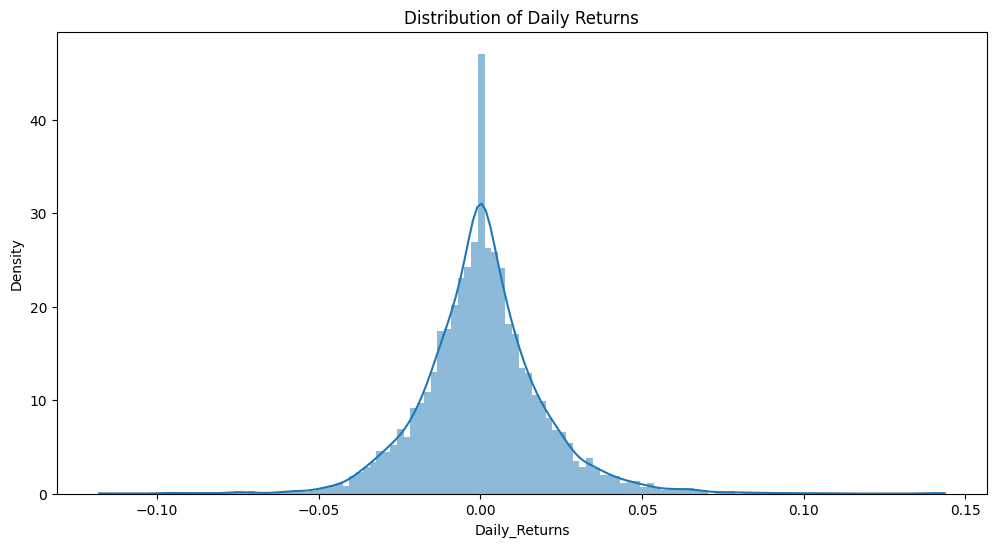
\includegraphics[scale=0.3]{stock_price_distribution.png}
    \caption{Histogram of the distribution of daily returns with a kernel density estimate overlay.}
    \label{fig:daily_returns}
\end{figure}

Figure \ref{fig:daily_returns} showcases the distribution of daily returns for Grupo Bimbo stock. It provides insights into the volatility and expected return, which are pivotal in risk assessment and portfolio management.

\begin{figure}[h!]
    \centering
    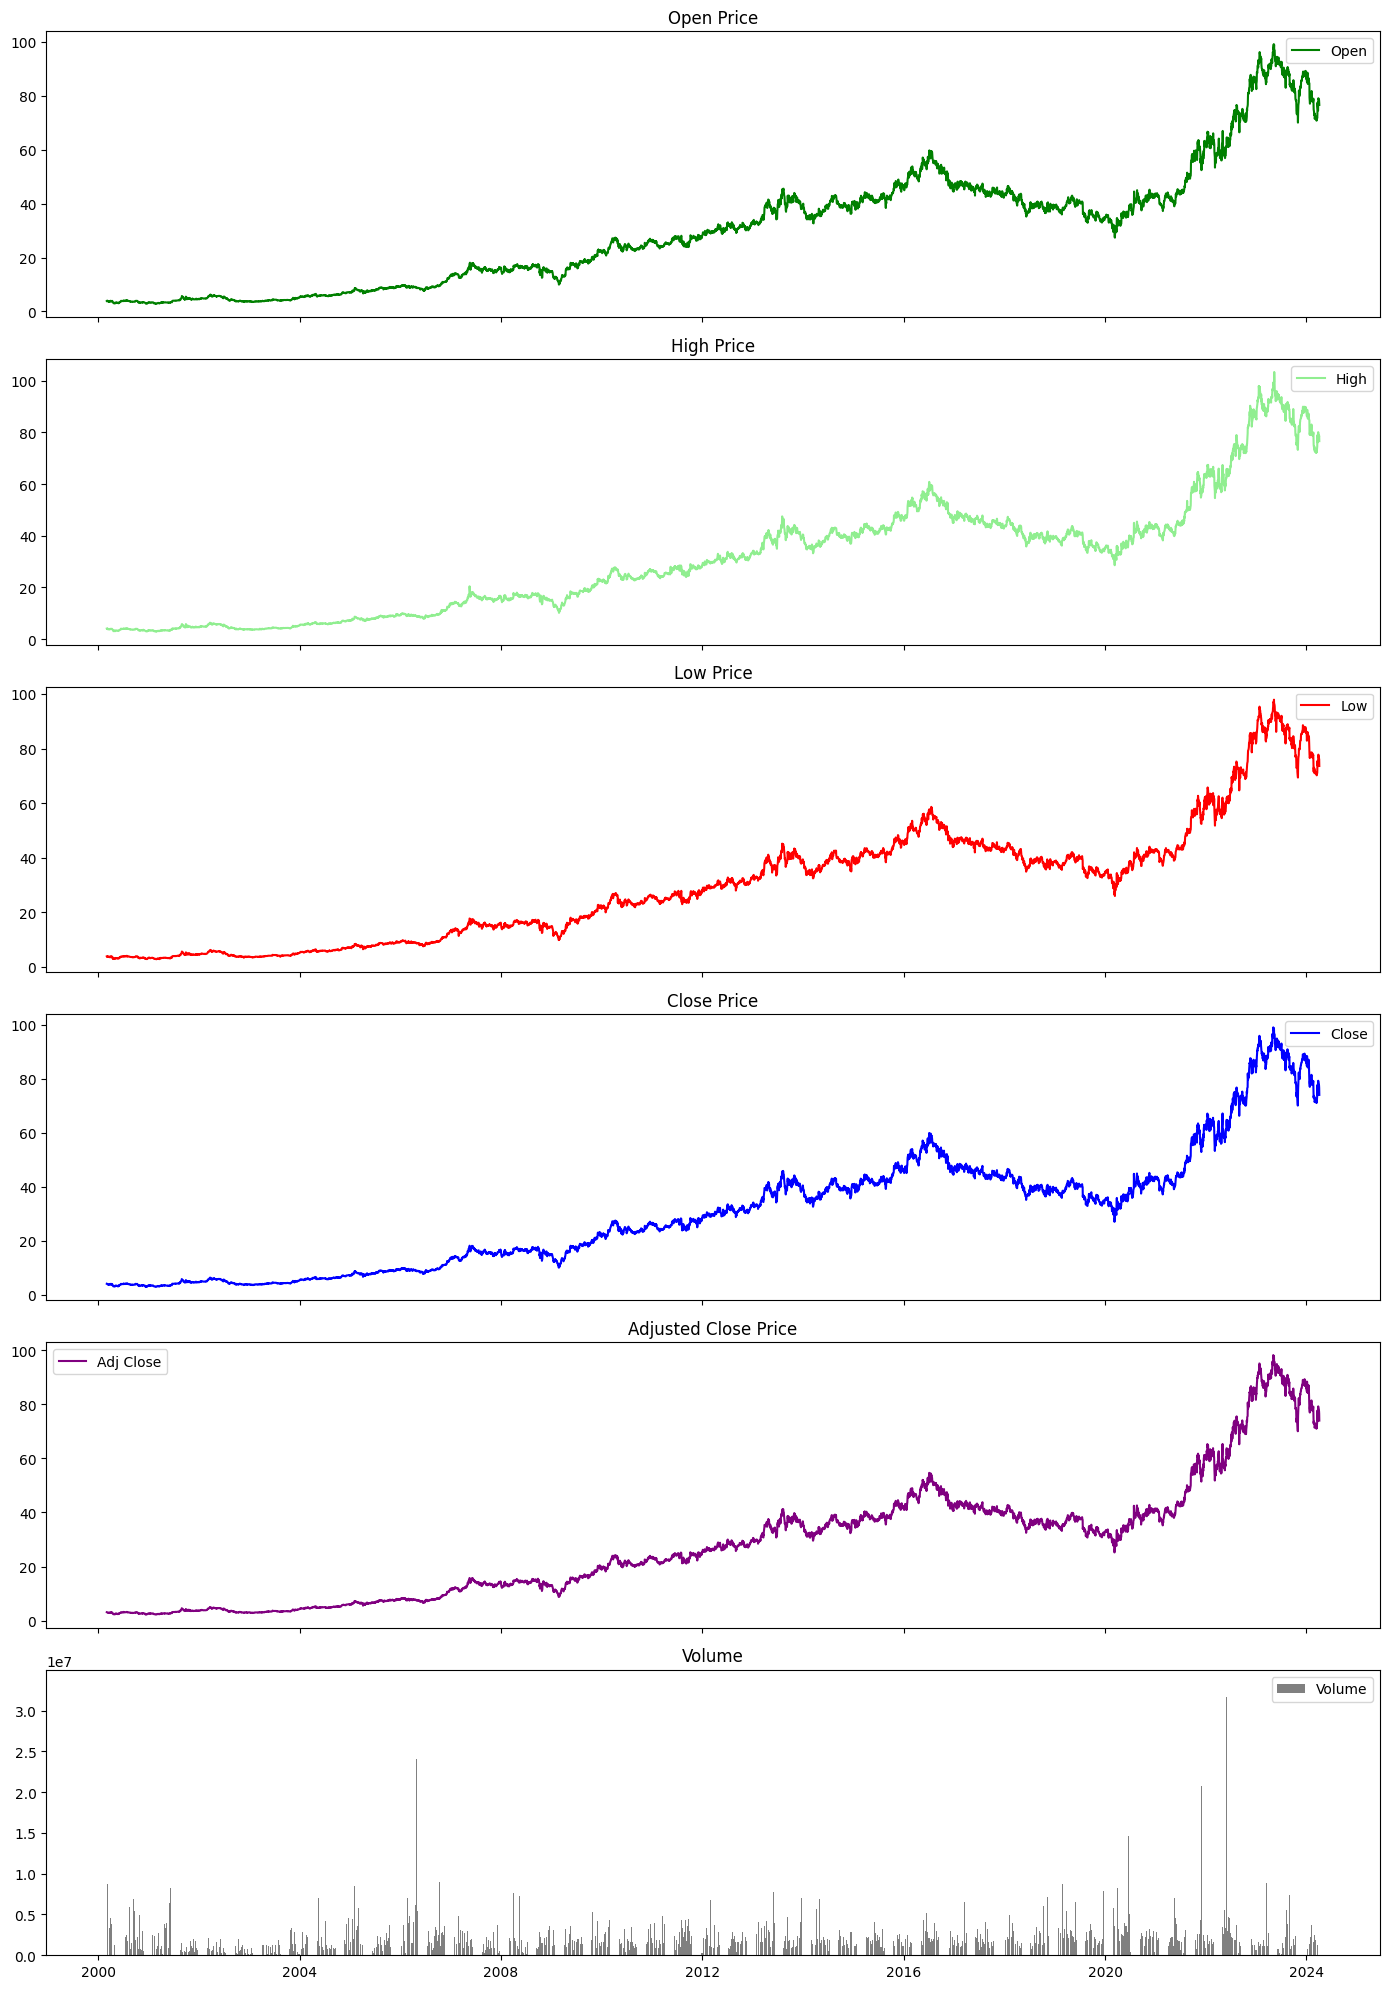
\includegraphics[scale=0.2]{stock_price.png}
    \caption{Time series data of the stock's open, high, low, close, adjusted close prices, and volume.}
    \label{fig:stock_price}
\end{figure}

Figure \ref{fig:stock_price} displays the stock's historical trading data, including open, high, low, close, and adjusted close prices. Additionally, the volume of shares traded is illustrated, which can be an indicator of market activity and liquidity.

Prior to predictive modeling, is necessary to know the distribution of the data. These visualizations provide a comprehensive view of the stock's historical performance and trading activity, which are valuable for both technical analysis and strategic planning in financial contexts.


\subsection{Predictive models}
Given the widespread use of advanced Machine Learning Techniques, Regressive Models, and SVMs in existing literature, our study aims to compare these well-established methods for predicting the stock prices of Grupo Bimbo.

\subsubsection{Auto Regressive Integrated Moving Average}

\begin{figure}
    \centering
    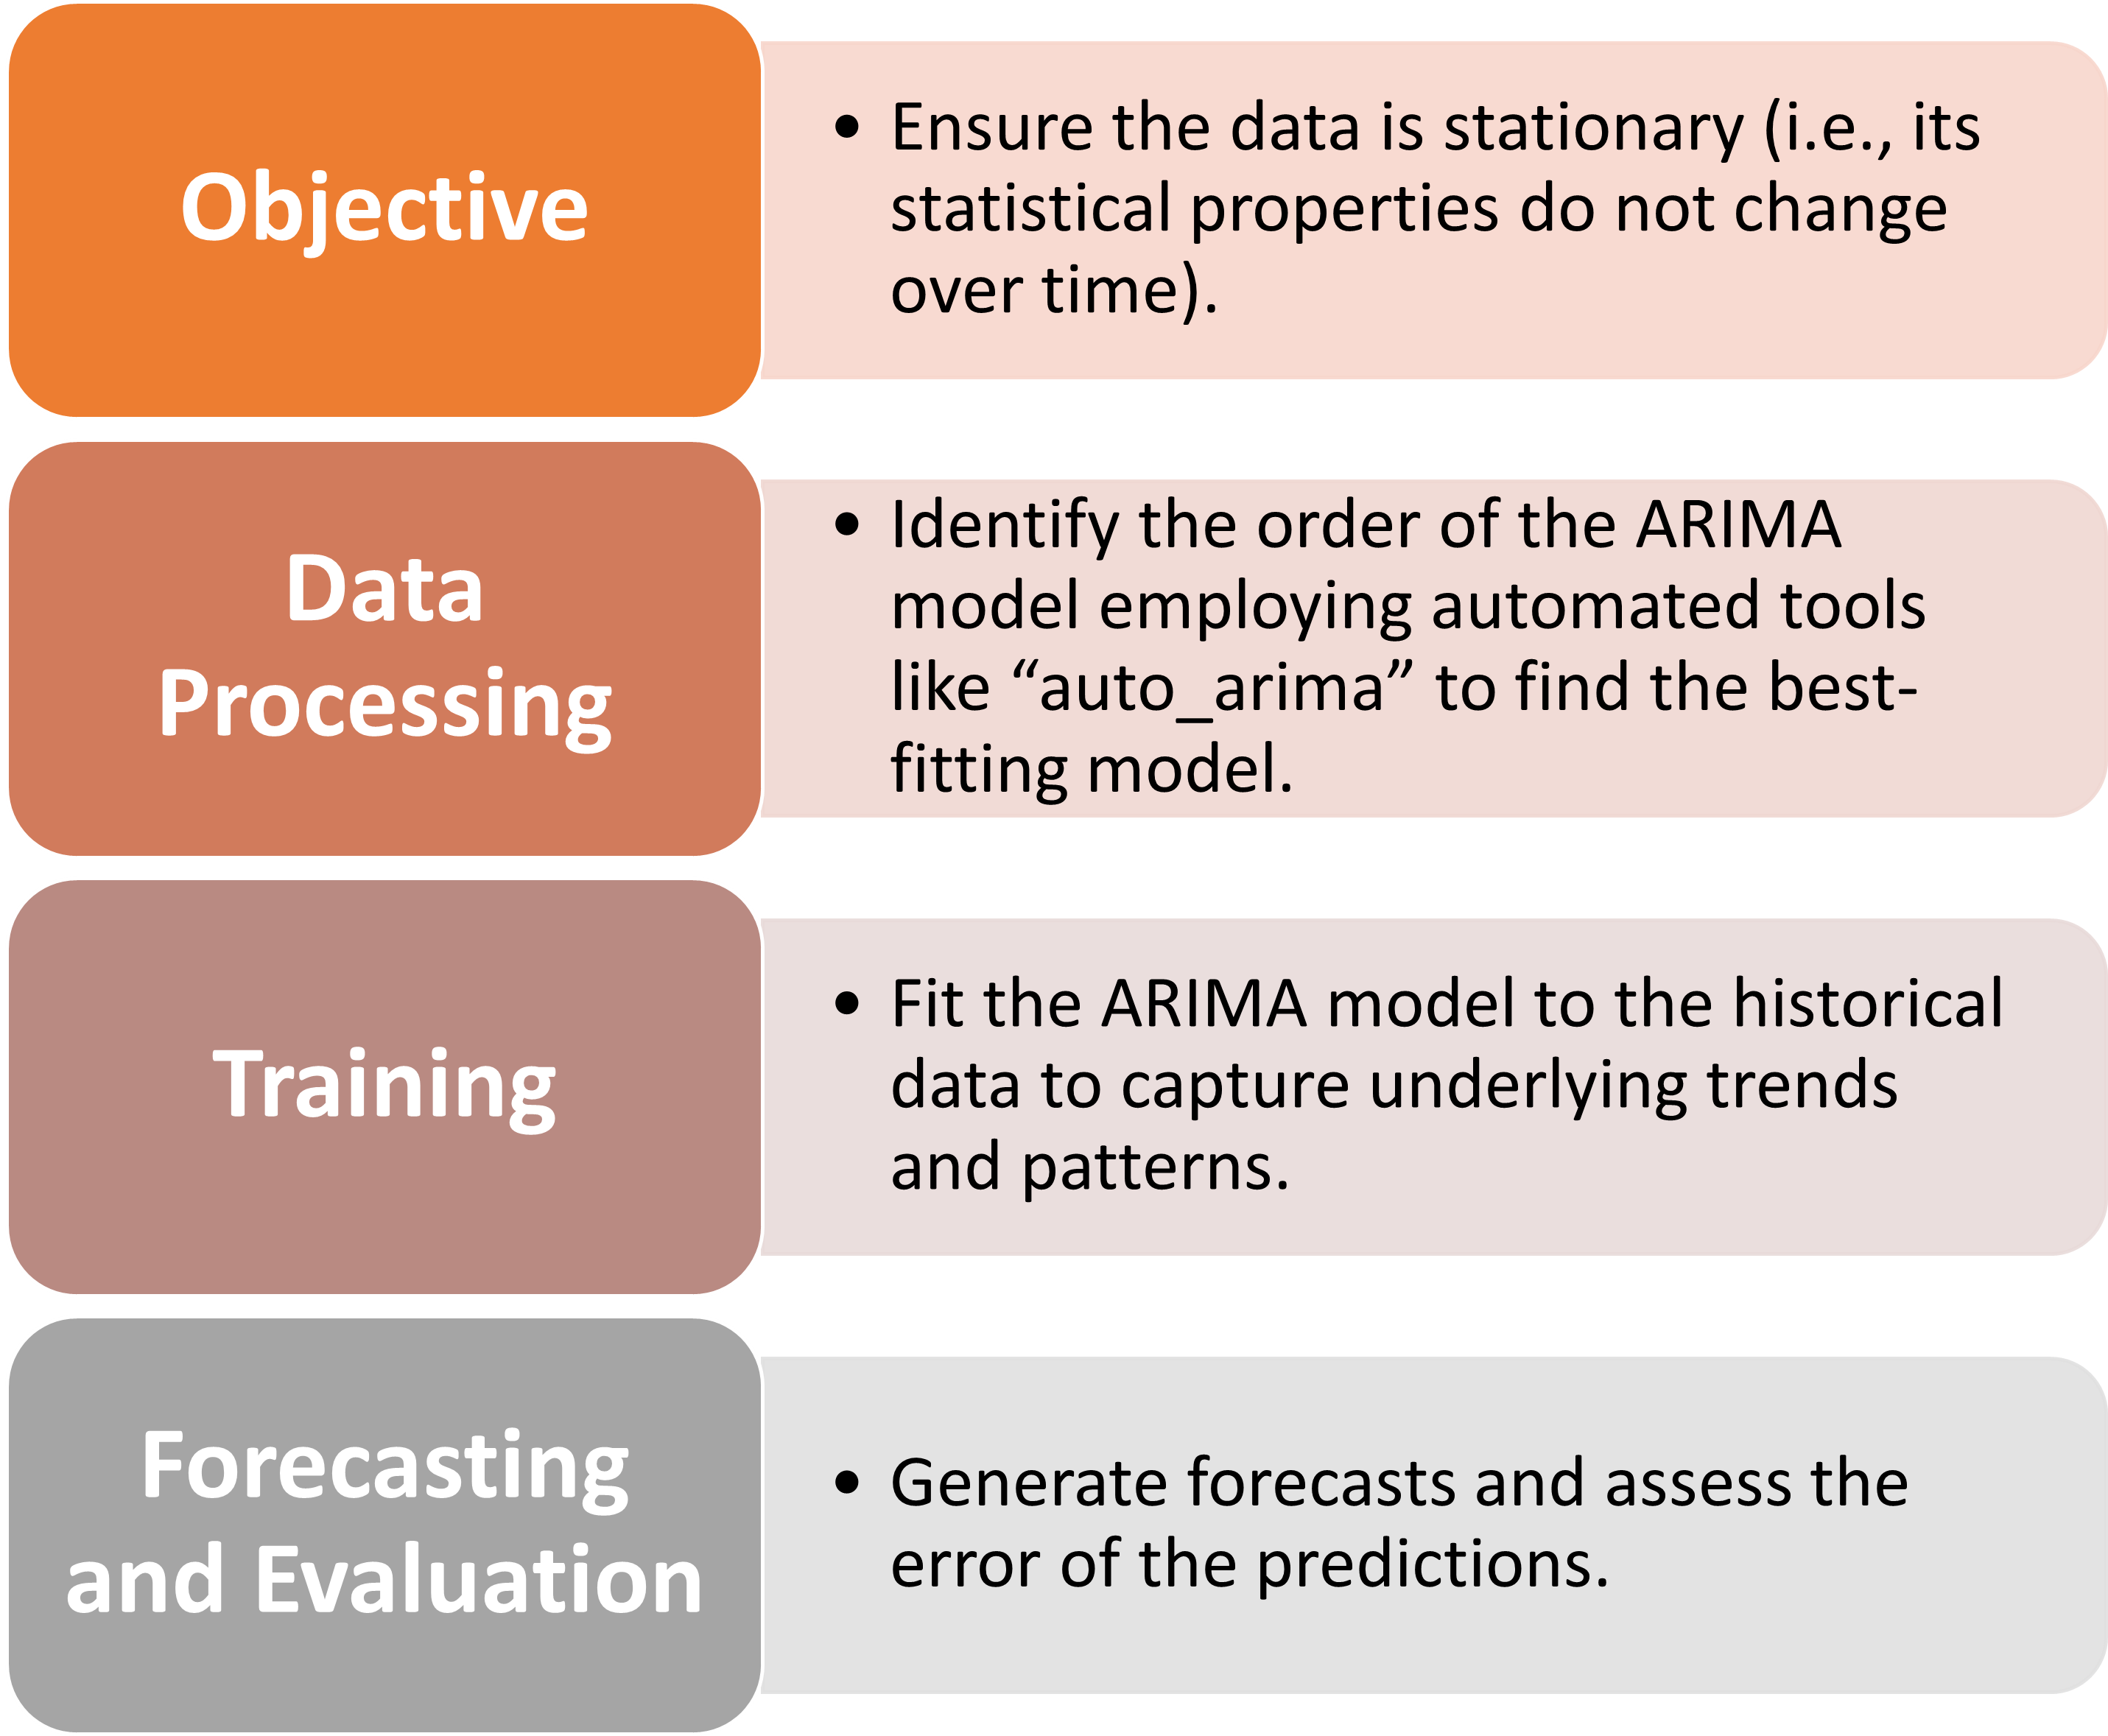
\includegraphics[scale=0.38]{flowARIMA.png}
    \caption{Flowchart ARIMA}
    \label{fig:enter-label}
\end{figure}

\subsubsection{Long-Short Term Memory}

\begin{figure}
    \centering
    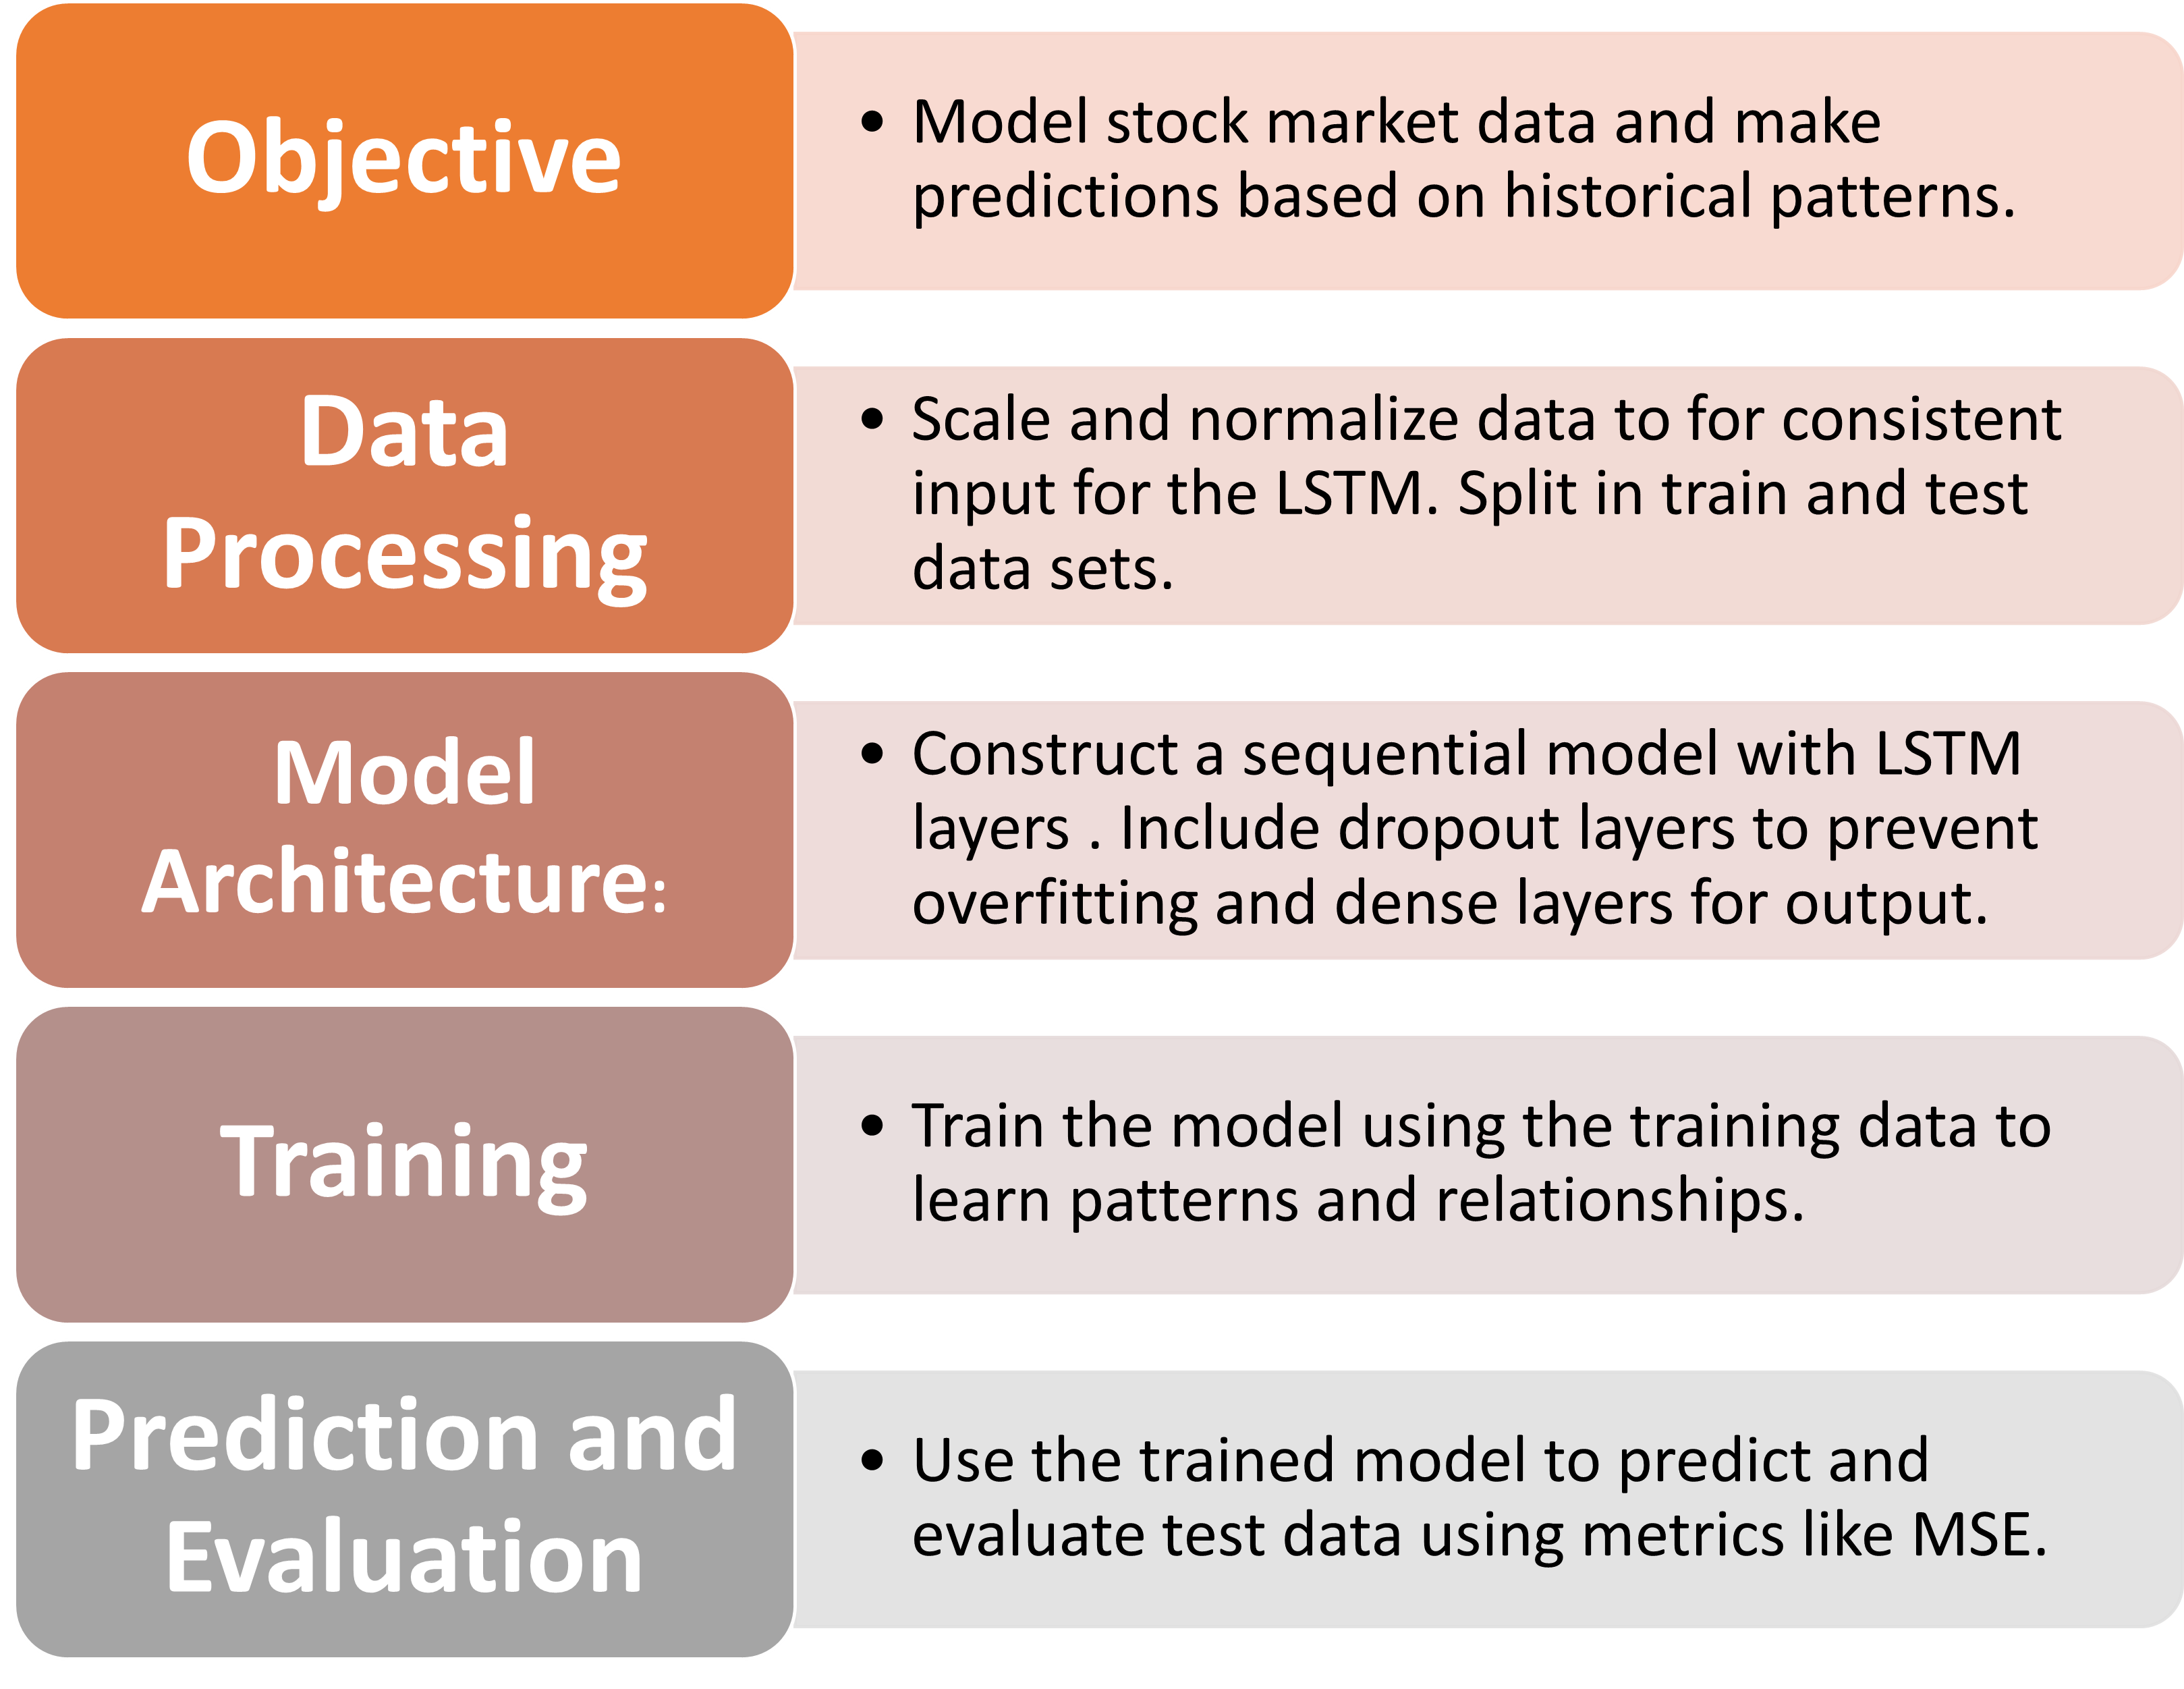
\includegraphics[scale=0.35]{flowLSTM.png}
    \caption{Flowchart LSTM}
    \label{fig:enter-label}
\end{figure}
\hspace{1pt}
For the LSTM the following architecture was developed:
\begin{itemize}
    \item Two LSTM layers with 64 units.
    \item One dense layer with 32 units
    \item One dropout layer with rate of 0.3
    \item One dense layer with 1 unit.
\end{itemize}
\subsection{Analytic Interactive Visualization}

Upon arrival to the descriptive results, a comprehensive business intelligence report including all the details will be presented. Such interactive dashboard report is hosted at the following link: \href{https://lookerstudio.google.com/reporting/cae0f4fa-54c3-483d-b90c-484b229ca1c7}{Interactive Dashboard Link}.

As shown in Figure \ref{fig:bimbostockprice}, the stock prices of Grupo Bimbo have experienced significant fluctuations over the years.

\begin{figure}[htbp]
    \centering
    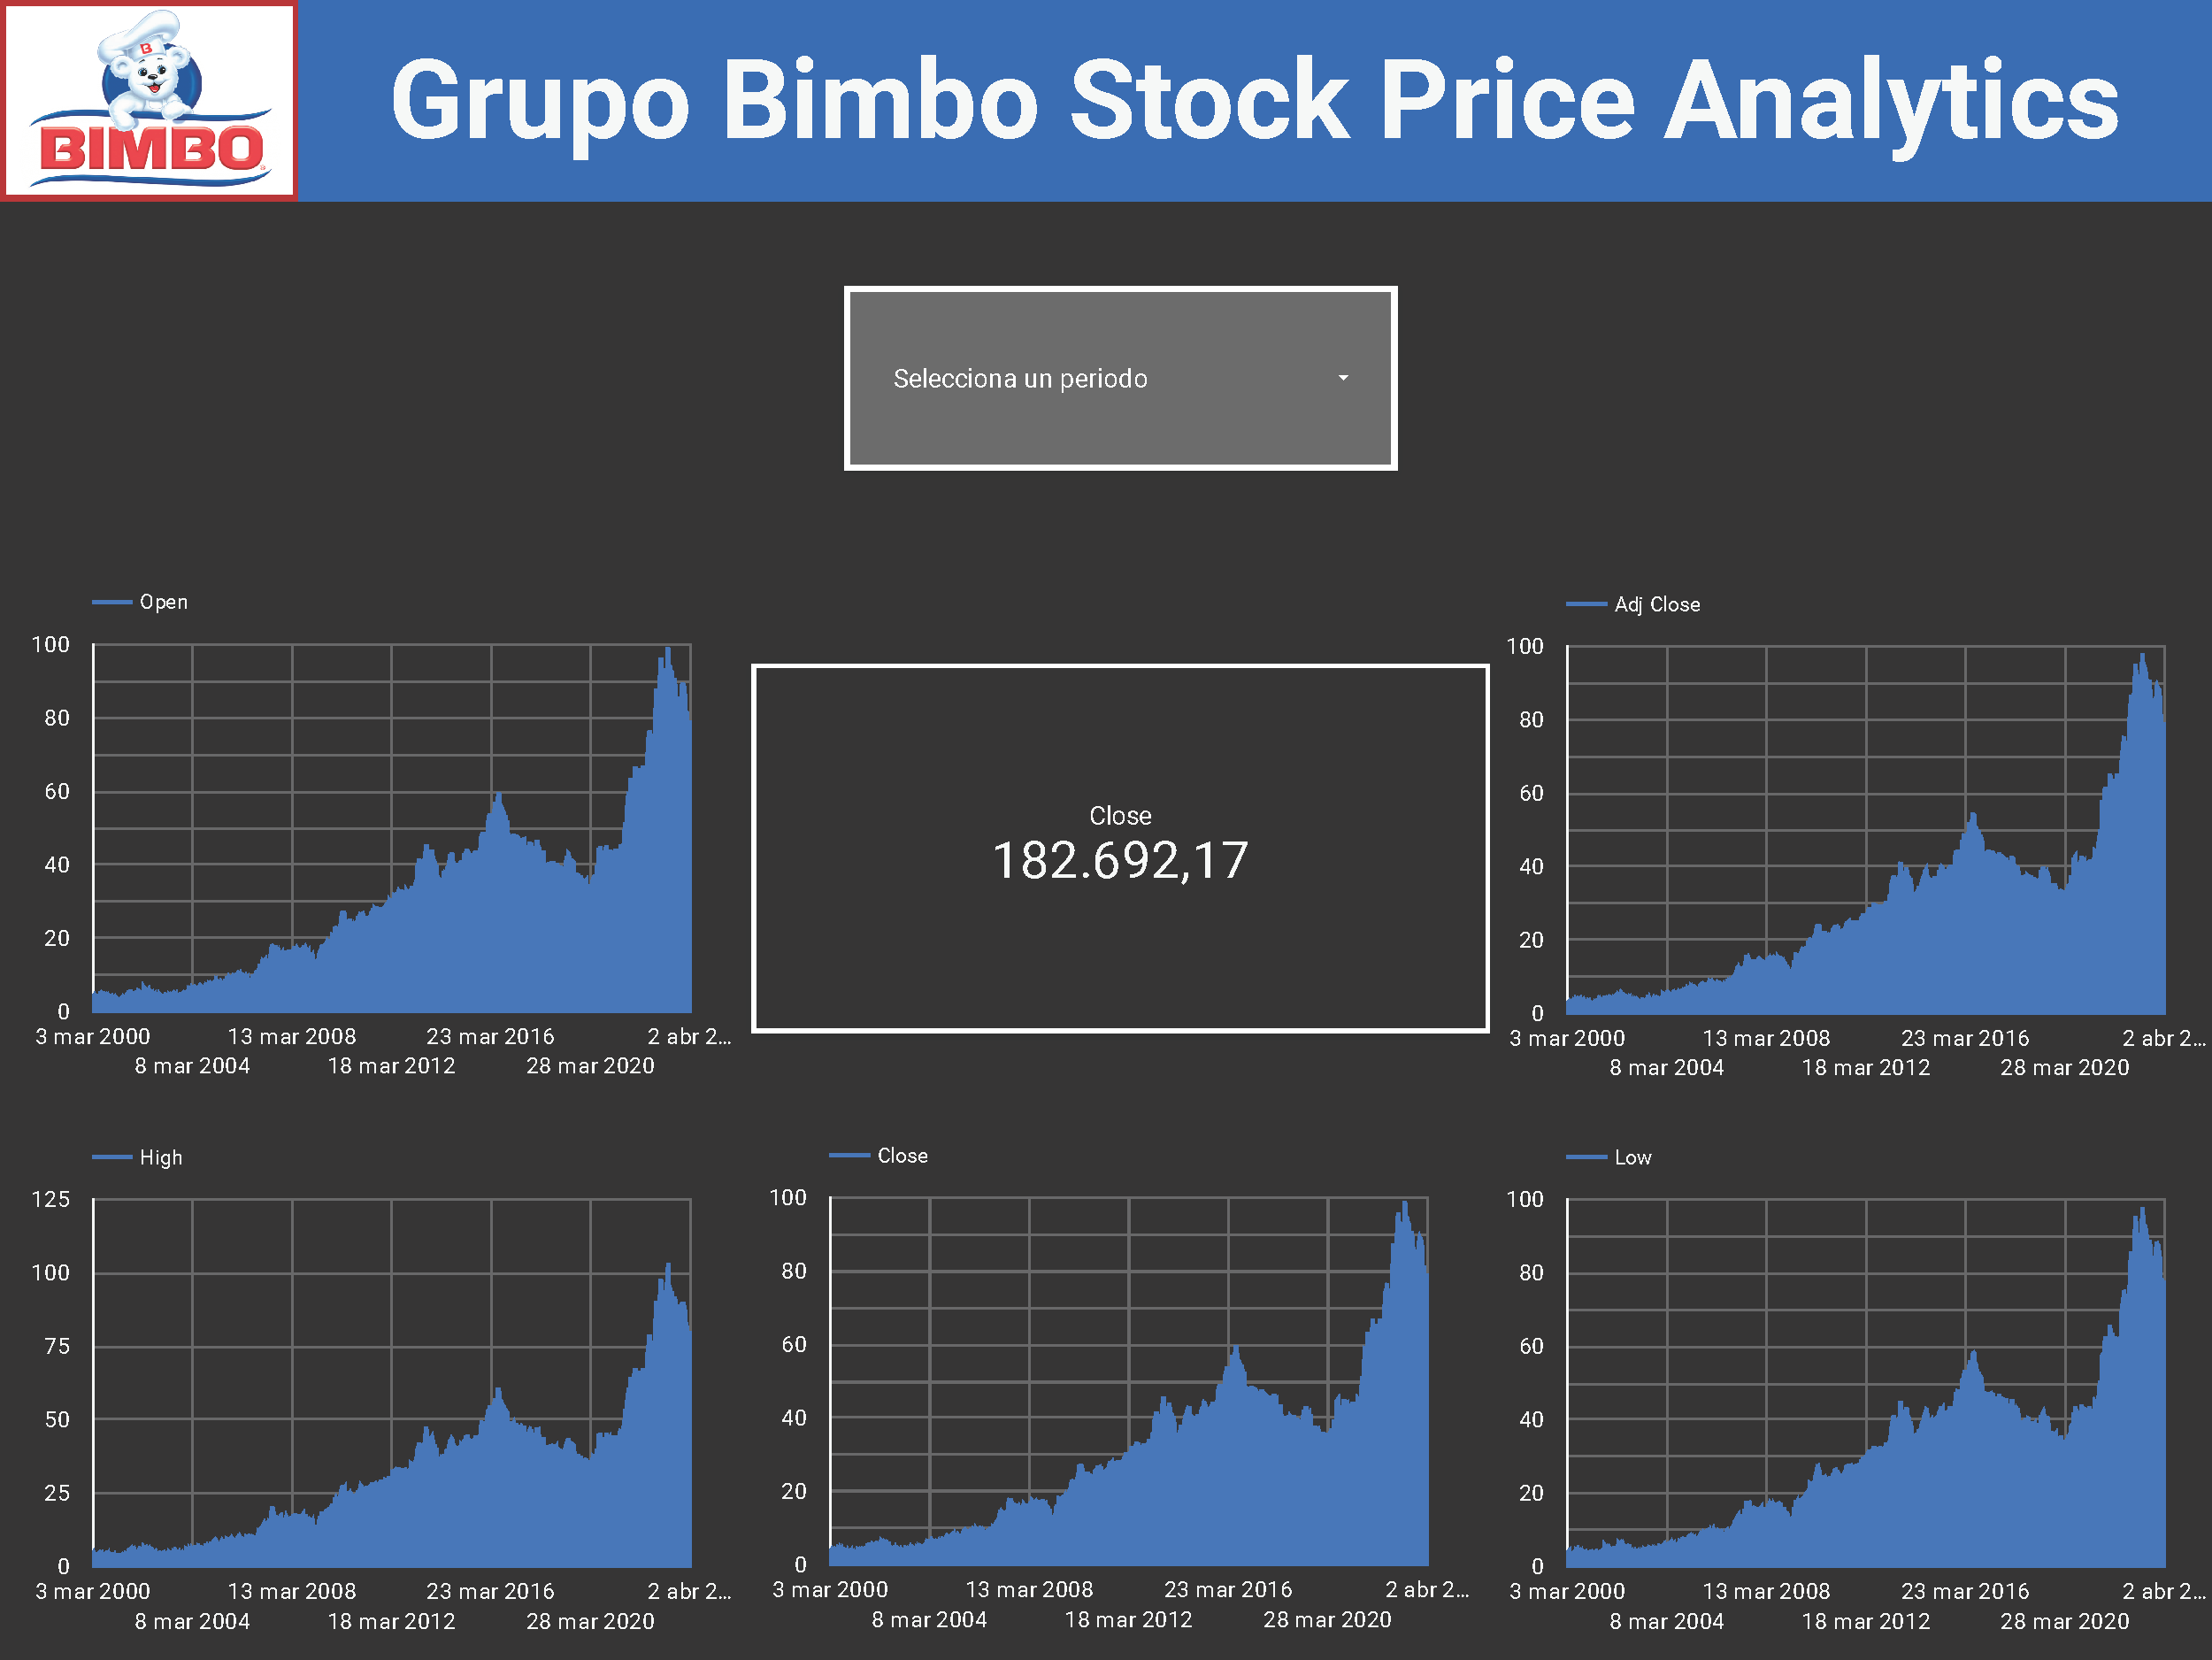
\includegraphics[scale=0.25]{Bimbo_Stock_Market_Dashboard_Preview.png} 
    \caption{Grupo Bimbo Stock Price Analytics, Business Dashboard Preview showing the historical stock price movement with opening, closing, high, low, and adjusted closing values.}
    \label{fig:bimbostockprice}
\end{figure}




\section{Results}

In our analysis of time series predictions for GRUPO BIMBO, we employed two different models: ARIMA and LSTM. 

Figure~\ref{fig:bimboarima} illustrates the forecasted values using the ARIMA model over 120 days. This model, known for its strength in capturing linear patterns and trends in time series data, provided a clear projection of future sales based on historical data. The ARIMA model's predictions indicate a steady trend with minor fluctuations, reflecting the inherent seasonal variations and trends in GRUPO BIMBO's sales data.

\begin{figure}[htb]
    \centering
    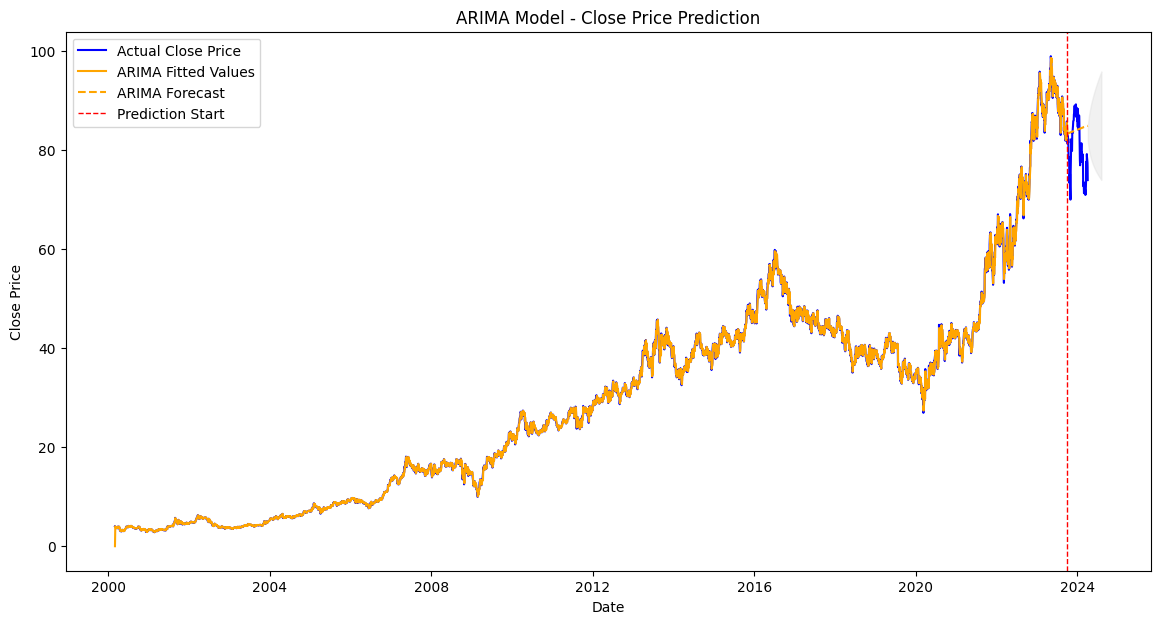
\includegraphics[scale = 0.3]{ARIMA.png}
    \caption{ARIMA Model Predictions: Time Series Forecast for GRUPO BIMBO Over a 120-Day Period}
    \label{fig:bimboarima}
\end{figure}

Conversely, Figure~\ref{fig:bibmolstm} showcases the predictions generated by the LSTM model for the same 120-day period. LSTM, or Long Short-Term Memory networks, is a type of recurrent neural network that is particularly effective in modeling complex, non-linear relationships within time series data. The predictions from the LSTM model exhibit a more dynamic range of fluctuations, capturing the intricate patterns and dependencies that might be present in GRUPO BIMBO's sales data. This approach allows for a nuanced understanding of the sales trends, potentially offering more precise insights into future sales behavior.


By comparing these two figures, we can observe how different modeling techniques can influence the forecasting results, thereby aiding in selecting the most suitable model for accurate and reliable predictions in time series analysis.

\begin{figure}[htb]
    \centering
    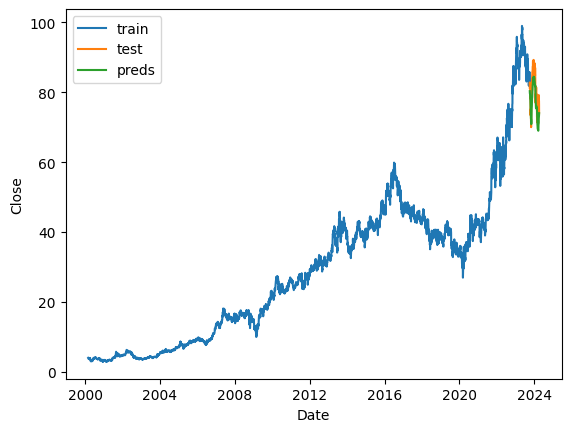
\includegraphics[scale = 0.6]{LSTM.png}
    \caption{LSTM Model Predictions: Time Series Forecast for GRUPO BIMBO Over a 120-Day Period}
    \label{fig:bibmolstm}
\end{figure}


\begin{table}[h!]
    \centering
    \begin{tabular}{|c|c|c|}
        \hline
        \textbf{Model} & \textbf{Specifications} & \textbf{MSE}  \\
        \hline
        ARIMA & (2,1,4) & 40.198 \\
        LSTM & ADAM Optimizer, 10 epochs, 0.01 LR.& 15.213\\
         \hline
    \end{tabular}
    \caption{Comparison between the LSTM model and the ARIMA model for 120 forecast. Long-Short Term Memory (LSTM), Autoregressive Integrated Moving Average (ARIMA)  Mean Standard Error (MSE), Learning Rate (LR).}
    \label{tab:my_label}
\end{table}

\section{Discussion}

In our comparative analysis of time series prediction models for GRUPO BIMBO, we explored the effectiveness of two distinct approaches: ARIMA and LSTM. Each model was evaluated over a 120-day forecasting period to determine its strengths and suitability for predicting sales data.

The ARIMA model, as depicted in Figure~\ref{fig:bimboarima}, is traditionally recognized for its proficiency in identifying and leveraging linear patterns within time series data. The forecasts generated by ARIMA revealed a stable trend with minor fluctuations, capturing the seasonal variations and trends inherent in GRUPO BIMBO's sales data. This model's ability to provide clear and straightforward projections makes it a valuable tool for understanding linear trends and patterns over time.

On the other hand, the LSTM model, shown in Figure~\ref{fig:bibmolstm}, offers a more sophisticated approach by capturing complex, non-linear relationships within the data. The LSTM model's predictions displayed a more dynamic range of fluctuations, reflecting the model's capability to account for intricate patterns and dependencies that are potentially present in the sales data. This characteristic of LSTM allows for a more nuanced understanding of sales trends, potentially offering deeper insights into future sales behaviors.

The juxtaposition of these models underscores the impact of different modeling techniques on forecasting outcomes. While ARIMA provides a more linear and stable forecast, the LSTM model offers a richer, more detailed view of potential future sales patterns. This comparison highlights the importance of selecting the appropriate model based on the specific characteristics of the data and the forecasting objectives.
\section{Conclusion}

In our analysis of GRUPO BIMBO's sales predictions over a 120-day period, we compared the ARIMA and LSTM models. The ARIMA model captured linear patterns and provided stable forecasts, reflecting seasonal variations. In contrast, the LSTM model excelled in modeling complex, non-linear relationships, resulting in more dynamic and accurate predictions.

The dataset used was extensive, which likely influenced the superior performance of the LSTM model. The Mean Squared Error (MSE) for ARIMA was 40.2, while LSTM achieved a significantly lower MSE of 15.21, indicating LSTM's greater accuracy in forecasting GRUPO BIMBO's sales.

Our study also highlighted the overall effectiveness of ANNs like LSTM in stock price prediction, especially with high-quality training data. ANNs outperformed autoregressive models such as ARIMA.

In summary, both models delivered acceptable predictions, but the LSTM model proved to be more accurate and effective. Leveraging LSTM can enhance GRUPO BIMBO's sales forecasting, supporting better decision-making and showcasing the model's practical application in predicting stock prices.

\begin{thebibliography}{00}

\bibitem{Mukherjee2021}Mukherjee, S. , et al.: Stock market prediction using deep learning algorithms. CAAI Trans. Intell. Technol. 8(1), 82–94 (2023). https://doi.org/10.1049/cit2.12059
\bibitem{Rouf2021}Rouf, N., Malik, M.B., Arif, T., Sharma, S., Singh, S., Aich, S., Kim, H.: Stock Market Prediction Using Machine Learning Techniques: A Decade Survey on Methodologies, Recent Developments, and Future Directions. Electronics 2021, 10, 2717. https://doi.org/10.3390/electronics10212717
\bibitem{Thakkar2021}Thakkar, A. \& Chaudhari, K. Fusion in stock market prediction: A decade survey on the necessity, recent developments, and potential future directions. Inf. Fusion 65, 95–107 (2021).
\bibitem{kumar2022} Kumar, D., Sarangi, P. K., \& Verma, R. (2022). A systematic review of stock market prediction using machine learning and statistical techniques. Materials Today: Proceedings, 49, 3187–3191. https://doi.org/10.1016/J.MATPR.2020.11.399

\bibitem{Nabipor2020}Nabipour M, Nayyeri P, Jabani H, Mosavi A, Salwana E, S. S. Deep Learning for Stock Market Prediction. Entropy. 2020; 22(8):840. https://doi.org/10.3390/e22080840
\bibitem{Long2020}Long, J., Chen, Z., He, W., Wu, T., \& Ren, J. (2020). An integrated framework of deep learning and knowledge graph for prediction of stock price trend: An application in Chinese stock exchange market. Applied Soft Computing, 91, 106205. https://doi.org/10.1016/J.ASOC.2020.106205
\bibitem{Jiang2021}Jiang, W. (2021). Applications of deep learning in stock market prediction: Recent progress. Expert Systems with Applications, 184, 115537. https://doi.org/10.1016/J.ESWA.2021.115537
\end{thebibliography}
\end{document}
